  %%%%%%%%%%%%%%%%%%%%%%%%%%%%%%%%%%%%%%% -*- coding: utf-8; mode: latex -*- %%
  %
%%%%%                         CHAPTER
 %%%
  %

% $Id: 2300-omnis-iste-natus.tex,v 1.2 2007/11/23 10:14:54 david Exp $
% $Log: 2300-omnis-iste-natus.tex,v $
% Revision 1.2  2007/11/23 10:14:54  david
% Bug fixes galore.
%
% Revision 1.1  2007/11/23 09:52:42  david
% *** empty log message ***
%
%

  %%%%%%%%%%%%%%%%%%%%%%%%%%%%%%%%%%%%%%%%%%%%%%%%%%%%%%%%%%%%%%%%%%%%%%%%%%%%%
  %
%%%%%                     HEAD MATTER
 %%%
  %

\chapter{Namespace Operation Performance Assessment}
%\addcontentsline{lof}{chapter}{\thechapter\quad Irure Dolor}
%\addcontentsline{lot}{chapter}{\thechapter\quad Irure Dolor}
\label{ch:Assessment}

 As this thesis is developed based on transactional framework of the second version (we called it PCC version) of Hop-HDFS, we will give a systematic namespace operation performance assessment between PCC and original HDFS in this section. All the tests are performed under same the experimental testbed described in Chapter~\ref{ch:evaluation} Section~\ref{sec:testbed}.

\section{NameNode Throughput Benchmark}

A \textit{NNThroughtBenchmark}~\cite{shvachko2010hdfs} tool has been developed to measure the NameNode performance. It is included in the Apache HDFS test package. The one used in this assessment is basically based on the code from Apache Hadoop HDFS 2.0.4 Aplha (We integrate the code which tests \textit{mkdirs} from HDFS 2.3.0 NNThroughtBenchmark into this one).

\noindent \textit{NNThroughtBenchmark} starts a NameNode and runs multiple client threads on the same node.  The same NameNode operation is performed by each client repetitively via directly calling the implemented NameNode method. The number of operations performed by the NameNode per second is measured.

\noindent In this section, we aims to give a performance comparison overview between HDFS and PCC. Since the workload is generated from a single machine by the \textit{NNThroughtBenchmark}, we set the number of operations to be 100 and the number of threads to be 3. For operations \textit{create, delete and rename}, the total number of files involved is 100. They are placed under 4 different directories equally. For operation \textit{mkdirs}, the total number of directories created is 100 and they are also placed under 4 different directories equally. See Figure~\ref{fig:nntp} for the operation performance comparison between HDFS and PCC (Hop-HDFS).

\begin{figure}[h]
	\centering
	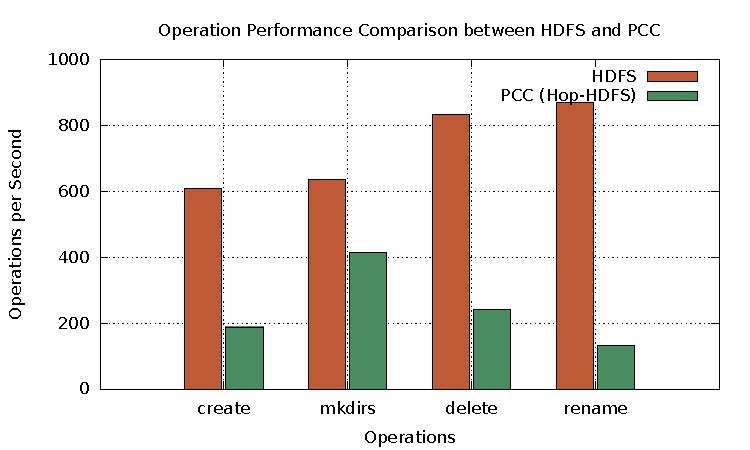
\includegraphics[width=\linewidth]{figs/nn_100.pdf}
	\caption{Operation Performance Comparison between HDFS and PCC (Hop-HDFS)}
	\label{fig:nntp}
\end{figure}

\noindent From Table~\ref{table:nntpb}, we find that the throughput of \textit{mkdirs} in PCC (Hop-HDFS) is 64.9 \% of HDFS, while others are all less than 30\%. The reason why \textit{create, delete and rename} is even worse is because they involve multiple NameNode primitive operations. For example, to finish \textit{create} operations, it took two NameNode primitive operations: \textit{startFile} and \textit{completeFile}. Since each NameNode primitive operation is implemented as a single transaction in Hop-HDFS, the more primitive operations involved, the more parent write locks will be, which means that more transactions will be blocked.
\begin{table}[h]
	\centering
	\begin{tabular}{|c|c|c|c|c|}
		\hline
		\textbf{Operations per Second} & \textbf{create} & \textbf{mkdirs} & \textbf{delete} & \textbf{rename} \\ \hline
		HDFS                           & 609             & 636             & 833             & 869             \\ \hline
		PCC (Hop-HDFS)                 & 188             & 413             & 242             & 132             \\ \hline
		PCC / HDFS              & 30.9\%          & 64.9\%          & 29.1\%          & 15.2\%          \\ \hline
	\end{tabular}
	\caption{Operation Performance Comparison between HDFS and PCC (Hop-HDFS)}
	\label{table:nntpb}
\end{table}